\chapter{Sentiment analysis and personality trait detection}
\textbf{John Culnan}
\section{Introduction}

Personality trait detection, sentiment analysis, and related measures of
personal characteristics like emotion recognition are all frequently used to
automatically gain an understanding of an object of study. As such, they
provide an AI agent with information about the background and states of
individuals at any given time, which may be used to allow the agent to interact
with individuals in a manner appropriate to their current state. Because
understanding the personalities and emotional states of other individuals is a
key feature of collaboration among people, it is a critical component of the
identification the overall mental states of others as required for a machine
theory of mind (e.g. \citet{Rabinowitz.ea:2018}). Providing an AI agent with
such ability will likewise help to inform a machine theory of teamwork by
allowing the AI agent to incorporate a wider range of key information in
performing its own role. 

There are no existing state of the art models for this particular dataset, as
it does not yet exist; however, state of the art models exist for related
datasets and tasks, some of which are incorporated into our model as
task-specific training data. For the Multimodal Emotion Lines Dataset
\citep{Poria.ea:2019}, which consists of a sentiment analysis task and a discrete
emotion recognition task, the state of the art model is TODKAT
\citep{Zhu.ea:2021}, which uses context-aware text and audio
transformer-based models for the emotion recognition task. The First
Impressions V2 dataset \citep{Ponce-Lopez.ea:2016}, consisting of the Big Five
personality trait classification for YouTube clips, was originally created for
use with a regression task; as a dominant trait classification task, the state
of the art model is \citet{Culnan.ea:2021}. The Multimodal Opinion-Level
Sentiment Intensity (MOSI) dataset \citep{Zadeh.ea:2016} consists of single
speakers in YouTube clips providing opinions that are rated from highly
negative to highly positive. The current state of the art model for MOSI is
TupleInfoNCE \citep{Liu.ea:2021}, which uses contrastive learning on
augmented data. 

One major limitation of current state of the art approaches is that the data
on which they are trained is not varied in source; typically, each task is
trained separately, so that when two or more tasks have similar or the same
label spaces, the model is retrained for each new task. The data within a
given task generally includes speakers with the same native language.
Multi-party data furthermore frequently come from scripted sources, such as
the television show Friends \citep{Poria.ea:2019, Zhu.ea:2021}), and single party
data from YouTube \citep{Zadeh.ea:2016, Ponce-Lopez.ea:2016}). Finally, these
state of the art models are created around datasets that rely on accurate,
hand-crafted transcriptions of the audio data, without considering
imperfections in the transcriptions. We approach this challenge by examining
the Study 3 data through multitask neural networks that make use of both
existing corpora as pre-training data as well as the Study 3 data to perform
the same tasks in a new domain, further seeking to improve performance by
giving special consideration to the imperfection of automatic ASR
transcriptions used with the Study 3 data. 


\section{Approach}

Our approach includes a hard parameter sharing multitask model pre-trained on
tasks for sentiment \citep{Zadeh.ea:2016}), emotion \citep{Poria.ea:2019}),
personality \citep{Ponce-Lopez.ea:2016}), and emotional intensity
\citep{Livingstone.ea:2018}), then trained on data from Study 3. Like Liu and
colleagues \citep{Liu.ea:2021}), our model will make use of augmented data to
allow for more balanced classes in each dataset of interest.  Acoustic and text
data will be fed into the model separately, with text data masked to handle
noise created by automatic transcription. These text transcriptions will be
paired in an ensemble with predictions made by a trained wav2vec model
\citep{Schneider.ea:2019}, which will allow for further boosting of text
modality accuracy. Acoustic and text data will subsequently be concatenated
prior to making predictions about the classes for each utterance-level data
point. A schematic representing our approach is shown in Fig
\ref{fig:sentiment_model_schematics}. 

\begin{figure}
    \begin{sidecaption}{Schematic representation of our multitask model}
    \centering
    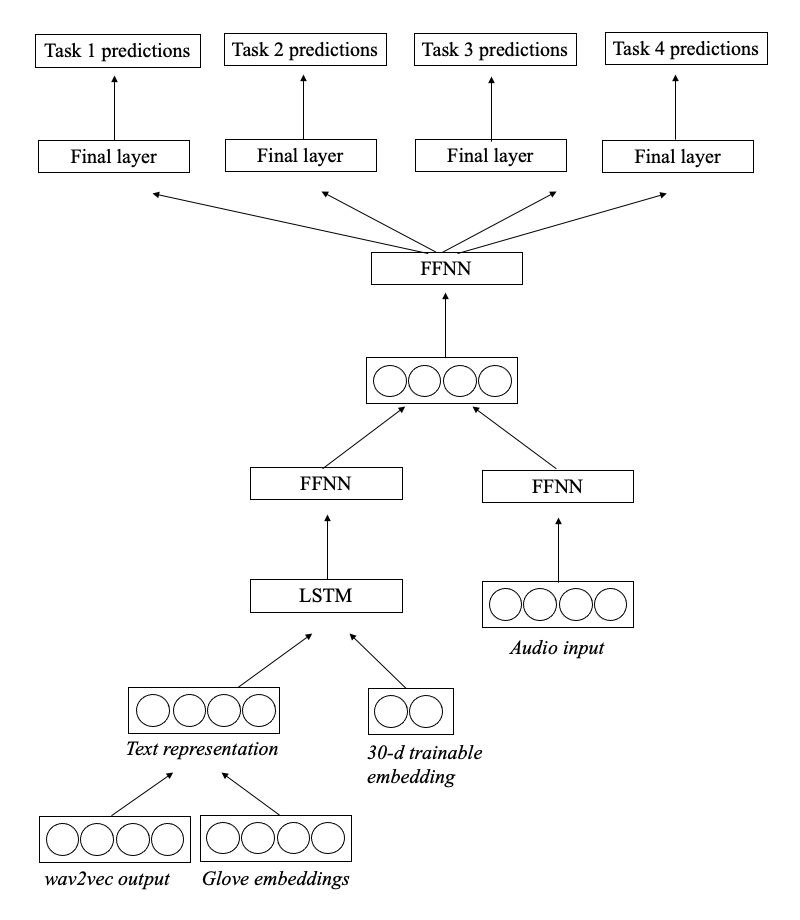
\includegraphics[width=\textwidth]{images/sentiment_schematics_study3.png}
    \label{fig:sentiment_model_schematics}
    \end{sidecaption}
\end{figure}

The study 3 data that will be incorporated into our models are the
pre-experiment TIPI survey
(Participant\_CognitiveTenItemPersonalityInventory\_Survey\_PreExperiment),
the text output of the ASR system
(MinecraftEntity\_Observation\_Asr\_Speechanalyzer), the audio data and the
acoustic features extracted from this audio signal
(MinecraftEntity\_Observation\_Audio\_Speechanalyzer). In addition to this
previously collected data, new utterance-level annotations will be collected
for sentiment, emotion, and emotional intensity. The text output of the ASR
system and the acoustic features extracted from the signal will be used as
input data in the model, while the TIPI and new utterance-level annotations
will be used as gold labels to evaluate the performance of our model. 


\section{Evaluation}

System evaluation will consist of examinations of the network's ability to
make correct predictions about sentiment, emotion, and personality traits
using F1 scores calculated by comparing network predictions with survey
responses and human-annotated data as described above. To provide comparable
scores to existing models for these tasks, average F1 scores will be used,
calculated as the weighted average of the F1 score for each class in the task.
Bootstrap resampling (citation) will be used to provide statistical
comparisons among models created with this network, enabling the
identification of the best model. 

While F1 calculations provide information on the overall success rate of our
network, they are limited in their ability to identify areas of weakness. To
further evaluate the ability of our network to perform under the different
conditions available, a subset of incorrect data points will be examined.
Patterns of errors that demonstrate model weaknesses with a particular type of
data (such as difficulty correctly identifying neutral sentiment in male
voices) will be used to inform further iterations of network updates. 
